% !TeX encoding = UTF-8
% !TeX program  = xelatex

\documentclass[12pt,a4paper,openany,
               afrikaans,UKenglish,
               masters-t,goldenblock 
              ]{stb-thesis} 

%==== Language setup =================================================
\usepackage{babel}
\usepackage[utf8]{inputenc}%...................... Unicode input file format

%==== Math setup =====================================================
\usepackage{amsmath}%............................. Advanced math (before fonts)
%\usepackage{amssymb}%............................ AMS Symbol fonts

%==== Font setup (default is Computer Modern) ========================
\usepackage{iftex}
\ifxetex
    \usepackage[math-style=TeX,
                bold-style=TeX,
               ]{unicode-math}
    \setmainfont{Cambria}%........................ Unicode fonts  (Win)                
    \setsansfont[Scale=MatchLowercase]{Calibri}
    \setmonofont[Scale=MatchLowercase]{Consolas}
    \setmathfont{Cambria Math}
    \defaultfontfeatures{Ligatures=TeX}
    \let\bm\symbfit
\else
    \usepackage[utf8]{inputenc}%.................. Unicode file format
    \usepackage{textcomp}%........................ Additional text symbols
    \usepackage[T1]{fontenc}%..................... Type 1 outline fonts
    \usepackage{bm}%.............................. Bold math fonts
\fi
\normalfont

%==== Units and numbers ==============================================
\usepackage{siunitx}%............................. Unit, number and angle output
    \sisetup{detect-all = true, detect-family = true}
    \sisetup{%output-decimal-marker = {.} ,
             group-separator = {\,},
             number-unit-product = {\,},
             inter-unit-product = \mathord{\cdot},
             exponent-product = \mathord{\times},
             separate-uncertainty = true}
   
         
%==== Ref's, Bib's and Nomencl =======================================
\usepackage{stb-nomencl}%......................... List of symbols 
    \renewcommand*{\UnitLabel}[1]{~[\,$\unit{#1}$\,]}
\usepackage{stb-bib}%............................. Bibliography (natbib internally)
    \bibliographystyle{stb-bib-eng-a}
    \renewcommand\bibfont{\small}
    \renewcommand\bibsection{\chapter{\bibname}}

%==== Tables + Graphics + Color =====================================
\usepackage{array}%............................... Extended table defs 
    \setlength{\extrarowheight}{2pt}
\usepackage{longtable}%........................... Tables can break over pages
\usepackage{graphicx}%............................ Included graphics
\usepackage[font=small]{caption}%................. Customize captions  
\usepackage[table]{xcolor}%....................... Color setup + colortbl 
    
%==== Extra defs for template ========================================
\makeatletter
%---- TOC entries and case
    \addto{\captionsafrikaans}{\renewcommand\bibname{Lys van verwysings}}
    \addto{\captionsafrikaans}{\renewcommand\contentsname{Inhoudsopgawe}}
    \addto{\captionsafrikaans}{\renewcommand\listfigurename{Lys van figure}}
    \addto{\captionsafrikaans}{\renewcommand\listtablename{Lys van tabelle}}

    \addto{\captionsUKenglish}{\renewcommand{\bibname}{List of references}}
    \addto{\captionsUKenglish}{\renewcommand\contentsname{Table of contents}}
    \addto{\captionsUKenglish}{\renewcommand\listfigurename{List of figures}}
    \addto{\captionsUKenglish}{\renewcommand\listtablename{List of tables}}

%==== User Defs ======================================================
%
% Please insert user defined commands here
% and NOT in the document itself!
%

\makeatother

%==== Title Page =====================================================
\title{\bfseries
       \AorE{%-- Afrikaans ------------------------------------------
             Diskrete Element Modellering van 'n Vibrerende Skeurploeg\\[1ex]
             \normalfont\small\itshape
             (``Discrete Element Modeling of a Vibratory Subsoiler'')
            }{%-- English -------------------------------------------
             Discrete Element Modeling of a Vibratory Subsoiler}}

\author{J.\ Doe}{John Doe}

\degree{\AorE{MIng (Meg)}{MEng (Mech)}}
       {\AorE{Magister in Ingenieurswese (Meganiese)}
             {Master of Engineering (Mechanical)}}

\address{\AorE{%-- Afrikaans ----------------------------------------
        Departement Meganiese en Megatroniese Ingenieurswese,\\
        Stellenbosch Universiteit,\\
        Privaatsak X1, Matieland 7602, Suid Afrika.%
             }{%-- English ------------------------------------------
        Department of Mechanical and Mechatronic Engineering,\\
        Stellenbosch University,\\
        Private Bag X1, Matieland 7602, South Africa.}}

\faculty{\AorE{Fakulteit Ingenieurswese}%
              {Faculty of Engineering}}

\supervisor{Dr.\ D.N.J.\ Els}
\cosupervisor{Prof.\ J.\ Smith}

\setdate{3}{2023}

%\SetSponsor{The financial assistance of the National Research Foundation (NRF)
%    towards this research is hereby acknowledged. Opinions expressed and
%    conclusions arrived at, are those of the author and are not necessarily to
%    be attributed to the NRF.}


%==== Main Document ==================================================
\setcounter{secnumdepth}{3}
\setcounter{tocdepth}{2}
\raggedbottom
\begin{document}   

\frontmatter%---------------------------------------------------------                    
\TitlePage

\DeclarationDate{2023/02/10}
\DeclarationPage


\begin{abstract}[english]%===================================================
Vibrating a tillage tool is an effective way of reducing the draft force
required to pull it through the soil. The degree of draft force reduction is
dependent on the combination of operating parameters and soil conditions. It
is thus necessary to optimize the vibratory implement for different
conditions.

Numerical modelling is more flexible than experimental testing and analytical
models, and less costly than experimental testing. The Discrete Element
Method (DEM) was specifically developed for granular materials such as soils
and can be used to model a vibrating tillage tool for its design and
optimization. The goal was thus to evaluate the ability of DEM to model a
vibratory subsoiler and to investigate the cause of the draft force
reduction.

The DEM model was evaluated against data ...
\end{abstract}


\begin{abstract}[afrikaans]%=================================================
Om `n tand implement te vibreer is `n effektiewe manier om die trekkrag, wat
benodig word om dit deur die grond te trek, te verminder. Die graad van krag
vermindering is afhanklik van die kombinasie van werks parameters en die
grond toestand. Dus is dit nodig om die vibrerende implement te optimeer vir
verskillende omstandighede.

Numeriese modulering is meer buigsaam en goedkoper as eksperimentele
opstellings en analitiese modelle. Die Diskrete Element Metode (DEM) was
spesifiek vir korrelrige materiaal, soos grond, ontwikkel en kan gebruik word
vir die modellering van `n vibrerende implement vir die ontwerp en optimering
daarvan. Die doel was dus om die vermoë van DEM om 'n vibrerende skeurploeg
the modelleer, te evalueer, en om die oorsaak van die krag vermindering te
ondersoek.

Die DEM model was geïvalueer teen data ...
\end{abstract}

\chapter*{Acknowledgements}



\chapter*{Dedication}



% Use \chapter*{} before TOC
\tableofcontents
% Use \chapter{} after TOC

\listoffigures
\listoftables
\chapter{List of symbols}
% Use stb-nomenclature + siunitx

\begin{Nomencl}[1cm]
\NomGroup{Constants}%-----------------------------------------------
    \item[$L_0 = $] \qty{300}{mm}

\NomGroup{Variables}%-----------------------------------------------
    \item[$\mathit{Re}_\mathrm{\,D}$]
                       \UnitLine{Reynolds number (diameter)}{~}
    \item[$x$]         \UnitLine{Coordinate                }{m}
    \item[$\ddot{x}$]  \UnitLine{Acceleration              }{m/s^2}\\
    
    \item[$\theta$]    \UnitLine{Rotation angle            }{rad}
    \item[$\tau$]      \UnitLine{Moment                    }{N.m}

\NomGroup{Vectors and Tensors}%-------------------------------------
    \item[$\overrightarrow{\bm{v}}$] Physical vector, see equation ...

\NomGroup{Subscripts}%----------------------------------------------
    \item[$\mathrm{a}$] Adiabatic
    \item[$a$]          Coordinate

\end{Nomencl}

\begin{Nomencl}[1cm]
\NomGroup{Abreviations}%-----------------------------------------------
    \item[DEM] Discrete Element Method
    \item[FEA] Finite Element Analysis

\end{Nomencl}


\mainmatter%----------------------------------------------------------
\numberwithin{figure}{chapter}
\numberwithin{table}{chapter}

\chapter{Introduction}

\section{Background}

Starting from the big picture, gradually narrow focus down to this project and where this report fits in.

\section{Objectives}

The objectives of the project (in some cases the objectives of the report). If necessary describe limitations to the scope.

\section{Motivation}

Why this specific project/report is worthwhile.
\chapter{Literature review}

\section{Discrete element method }

The Discrete Element Method (DEM) analysis \citep{Cundall-1979} uses spherical objects. \citet{Lin:1997} developed a DEM model for ellipsoids.
\chapter{Content chapter}

Unless the chapter heading already makes it clear, an introductory paragraph that explains how this chapter contributes to the objectives of the report/project.

\section{Heading level 2}

\subsection{Heading level 3}

\subsubsection{Deepest heading, only if you cannot do without it}
\vspace{2cm}

\paragraph{Equations:}

An equation must read like part of the text. The solution of the quadratic equation $ax^2+bx+c=0$ given by the following expression (note the full stop after the equation to indicate the end of the sentence):
\begin{equation}
    x = \frac{-b \pm \sqrt{b^2-4ac}}{2b} .
\end{equation}
In other cases the equation is in the middle of the sentence. Then the paragraph following the equation should start with a small letter. Euler's identity is 
\begin{equation}
    e^{i \pi} + 1 = 0 ,
\end{equation}
where $e$ is Euler's number, the base of natural logarithms.

The \texttt{amsmath} has a wealth of structure and information on formatting of mathematical equations.

\pagebreak
\paragraph{Symbols and numbers:}

Symbols that represent values of properties should be printed in italics, but SI units and names of functions (e.g. sin, cos and tan) must not be printed in italics. There must be a small hard space between a number and its unit, e.g. \qty{120}{km}. Use the \texttt{siunitx} package to typeset numbers, angles and quantities with units:
\begin{tabbing}
\hspace*{\parindent}\=\verb|\qty{20}{N.m}|\quad\=$\rightarrow$\quad\=\kill
    \>\verb|\num{1.23e3}| \>$\rightarrow$\> $\num{1.23e3}$ \\
    \>\verb|\ang{30}|     \>$\rightarrow$\> $\ang{30}$ \\
    \>\verb|\qty{20}{N.m}|\>$\rightarrow$\> $\qty{20}{N.m}$
\end{tabbing}

\paragraph{Figures and tables:}
The \texttt{graphicx} package can import \texttt{PDF}, \texttt{PNG} and \texttt{JPG} graphic files.

\begin{table}[htbp]
    \centering
    \caption{Standard ISO paper sizes}
    \label{tab:paper}
    \begin{tabular}{lcccc}
    \hline
        Paper\quad && \multicolumn{3}{c}{Sizes} \\
    \cline{2-5}
        &&  $W$      && $H$ \\
        && \small [mm] &&  \small [mm]   \\
    \cline{1-1}\cline{3-3}\cline{5-5}
        A0 && 841 && 1189 \\
        A1 && 594 &&  841 \\
        A2 && 420 &&  594 \\
        A3 && 297 &&  420 \\
        A4 && 210 &&  297 \\
        A5 && 148 &&  210 \\
    \hline
    \end{tabular}
\end{table}


\begin{figure}[htbp]
    \centering
    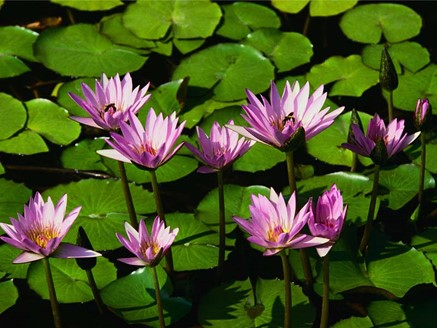
\includegraphics[scale=0.75]{figs/waterplants}
    \caption{Water plants}
    \label{fig:waterplant}
\end{figure}

\chapter{Conclusions}


\appendix%------------------------------------------------------------
\chapter{Mathematical proofs}

\section{Euler's equation}
Euler's equation gives the relationship between the trigonometric functions and the complex exponential function.
\begin{equation}
    e^{ i\theta } = \cos \theta + i\sin \theta
    \label{eq:Euler}
\end{equation}
Inserting $\theta=\pi$ in \eqref{eq:Euler} results in Euler's identity
\begin{equation}
    e^{ i \pi} + 1 = 0
    \label{eq:Euler2}
\end{equation}


\section{Navier Stokes equation}

The Navier–Stokes equations mathematically express momentum balance and conservation of mass for Newtonian fluids.  Navier-Stokes equations using tensor notation:
\begin{subequations}
\begin{gather}
    \frac{\partial \rho}{\partial t} +
    \frac{\partial}{\partial x_j}\left[ \rho u_j \right] = 0 
    \\
    \frac{\partial}{\partial t}\left( \rho u_i \right) +
    \frac{\partial}{\partial x_j}
    \left[ \rho u_i u_j + p \delta_{ij} - \tau_{ji} \right] = 0, \quad i=1,2,3
    \\
    \frac{\partial}{\partial t}\left( \rho e_0 \right) +
    \frac{\partial}{\partial x_j}
    \left[ \rho u_j e_0 + u_j p + q_j - u_i \tau_{ij} \right] = 0
\end{gather}
\end{subequations}

\chapter{Experimental results}


\backmatter%----------------------------------------------------------
\bibliography{bib/bib-sample}
 
\end{document}   

